% Created 2021-12-13 Mon 23:08
% Intended LaTeX compiler: xelatex
\documentclass[11pts]{article}
\usepackage{graphicx}
\usepackage{grffile}
\usepackage{longtable}
\usepackage{wrapfig}
\usepackage{rotating}
\usepackage[normalem]{ulem}
\usepackage{amsmath}
\usepackage{textcomp}
\usepackage{amssymb}
\usepackage{capt-of}
\usepackage{hyperref}
\usepackage[indent]{parskip}
\usepackage{indentfirst}
\usepackage[natbib=true]{biblatex}
\usepackage[margin=2cm]{geometry}
\usepackage{float}
\usepackage{algpseudocode}
\usepackage{algorithm}
\usepackage{graphicx}
\usepackage{setspace}
\onehalfspacing
\usepackage{fontspec}
\setmainfont{Times New Roman}
\author{CHOI Sen Hei 1155109412 \\
x}
\date{\today}
\title{RMSC4002 Project \\
Trading Strategy with PCA and Kelly's Formula \\
}
\hypersetup{
 pdfauthor={CHOI Sen Hei 1155109412 \\
x},
 pdftitle={RMSC4002 Project \\
Trading Strategy with PCA and Kelly's Formula \\
},
 pdfkeywords={},
 pdfsubject={},
 pdfcreator={Emacs 27.1 (Org mode 9.5)}, 
 pdflang={English}}
\begin{document}

\maketitle
\tableofcontents


\section{Introdution}
\label{sec:orgf312760}
Nowadays more and more people want to earn some money through investing in the stock market. There are various trading strategies which claim to generate profits but some of them fail if the market is performing worse. In this report, we aim at introducing a trading strategy that is able to outperform the market and reduce losses in economic downturns. The strategy is a combination of three components: stock selection by Principal Component Analysis (PCA), portfolio optimization, and a trading strategy called the Kelly's Formula. 
In the project, we used historical stock data from 2000 to 2021 to test the performance of the above trading strategy. There were some financial crises that happened during the selected period such as the crisis in 2007-2008, and the crisis in 2020. The test is performed by R programming. Details of the procedures and results are included in the following sections in this report.

\section{Method}
\label{sec:org6462d79}
\subsection{Dataset}
\label{sec:orge4ee10e}
Our research is based on US Stock Market. For the dataset, we obtained the price data from each component in Russell3000 from Bloomberg terminal. The daily adjusted open price of the components from 2000/01/01 - 2021/11/12 are then collected using the BDH function in the Excel add-in. Among 3041 stocks collected, 833 are shortlisted which provide complete data among the 22 years time period.
\subsection{Assumptions and Parameters}
\label{sec:orgdb0bad9}
\begin{enumerate}
\item 10000 USD is used as the principal
\item Only Long is available, no short sales
\item Commission per trade : max\{2.05, 1.3\% \texttimes{} number of stock traded \}
\item Window size of arithmetic return : 50-days
\item \(\lambda\)=0.94, estimated by J.P. Morgan Riskmetrics database(1)
\end{enumerate}

\subsection{Algorithm}
\label{sec:org1a922c5}
Library used:\\
\indent library(tseries)\\
\indent library(zoo)\\
\indent library(lubridate)\\
\indent library(fGarch)

The overall procedure in a nutshell is as follow:

\begin{enumerate}
\item The adjusted open price data is splitted into 2 parts, the first years data (2000) are implemented as the historical price used for the estimated volatility in GARCH(1,1) model and EWMA model, also an initial portfolio with ten stocks is formed by applying PCA selection to the first five years prices. The next 21 years data are then implement with the investment strategy described below
\item A trading strategy through Kelly's Formula would be applied to maximize the trading profit regarding the principle of buy-low and sell-high, based on the threshold of buying and selling will be described in the later section of the report
\item When the sell signal is triggered, all stocks we are holding will be sold and PCA is implemented to find out the other ten best-performing stocks from Russell 3000 based on the one-year historical data from the trigger time point. Then, portfolio optimization would be performed to find out the best weighting of the stocks to compose the portfolio. A mean-variance efficient portfolio can be obtained as the solution of minimizing the portfolio variance under the constraint that the portfolio expected return equals a target return.
\item When the buying signal is triggered, all cash in hand will be spent to buy the portfolio based on the latest PCA selection and hold the portfolio until the next selling signal is triggered.
\end{enumerate}
\begin{algorithm}[H]
\caption{Trading Strategy Algorithm}
\begin{algorithmic}[1]
\State \textbf{Input:} Stock price dataset $S_{t}, t = 1, 2, ..., T$.
\State Compute log-return $u_{t} = log(S_{t})-log(S_{t-1})$;
\State Apply PCA on first 252 days log-return: $u_{1:252}$;
\State Select top 10 stocks with highest loadings;
\State \textbf{Initialize:} Window size = 50, N Obs = 252, Initial Cash = 10000;
\For{$t \gets 252, T$}
\State GARCH(1,1):
\State $\sigma_{t}^{2} \gets \gamma V_{L}+\alpha u_{t-1}^{2} + \beta \sigma_{t-1}^{2}$;
\State $\mu_{t} \gets \frac{1}{50}\sum_{u_{t-50}}^{u_{t}}$;
\State Goodness GARCH $\alpha_{t} \gets \frac{\mu_{t}}{\sigma_{t}} - \frac{1}{2}$;
\State EWMA:
\State $\sigma_{t}^{2} \gets \lambda \sigma_{t-1}^{2}+(1-\lambda)u_{t-1}^{2}$;
\State $\mu_{t} \gets \frac{1}{50}\sum_{u_{t-50}}^{u_{t}}$;
\State Goodness EWMA $\alpha_{t} \gets \frac{\mu_{t}}{\sigma_{t}} - \frac{1}{2}$;
\If{t < 253}
\State Next;
\EndIf
\If{No stocks and $\alpha_{t-1} < 0$ and $\alpha_{t} > 0$}
\State Buy;
\ElsIf{Have stocks and $\alpha_{t-1} > 0$ and $\alpha_{t} < 0$}
\State Sell;
\State Update portfolio with PCA Algorithm;
\EndIf
\EndFor
\State \textbf{Return:} Values of each model;
\end{algorithmic}
\end{algorithm}

\subsection{PCA}
\label{sec:org1a19e45}
Principal Component Analysis (PCA) is a multivariate statistical technique for dimension reduction. It is commonly used for image processing and variable selection. 
In this project, PCA is applied to stocks in the Russell3000 index as a stock selection method to build a portfolio of 10 stocks that closely represents the index. PCA decomposes the interrelated variables into uncorrelated principal components. The first PC is used for variable selection as it is the major market factor. It can represent the financial market performance. We select the 10 stocks with highest loadings in the first PC. The stock selection method works together with Kelly's formula, so we used a rolling window approach. For each time we sell our stocks at time t, we will apply PCA on the past t-253 to t-1 log-return to update our portfolio.
Using PCA to extract the top 10 stocks can be obtained as follows: \\
Step 1 : Input stocks' price in the index, compute the log-return as u. \\
Step 2 : Calculate the covariance matrix of the first 252 days log-return u. Apply eigendecomposition on the covariance matrix, with eigenvalues \(\sigma\) and eigenvectors V. \\
Step 3 : Select the first PC which is the eigenvector with largest corresponding eigenvalue. Select the top 10 stocks with highest loadings in the first PC. \\
Step 4 : Repeat step 2 and step 3 with past 252 days log-return when sell signal is triggered. \\

The reason we use PCA for building our portfolio is that it is unwise to buy and hold a single stock. Building a portfolio with stocks in different sectors helps traders to diverse risk. Diversification is an important concept in investing. It prevents traders from losing all investment in a single asset. Variables selection by PCA will extract the uncorrelated components in the dataset.  The reason for including securities that have low correlations or even negative correlations in our portfolio is that they will eliminate some risk which has become known as idiosyncratic or diversifiable risk. PCA for stock selection gives a good level of diversification and a reasonable performance. Also, the portfolio with PCA selected stock will replicate the index behavior except the financial crisis during pandemic. And the rolling windows approach to apply PCA on different periods of time updates our portfolio that gives out better performance in that time period.

The algorithm of updating portfolio at today using the past 252 days log-return is shown below:
\begin{algorithm}[H]
\caption{PCA Algorithm}
\begin{algorithmic}[1]
\State \textbf{Input:} Date T, N stocks log-return vectors in past 252 days $u_{1},u_{2}, ... ,u_{N} \in \mathbb{R}^{252}$ .
\State Compute mean vector;
\State $\bar{u} \gets \frac{1}{N} \sum_{i=1}^{N}u_{i}$;
\State Subtract mean vector;
\For{$i \gets 1 , N$}
    \State $\Phi_{i} \gets u_{i} - \bar{u}$;
\EndFor
\State $A \gets [\Phi_{1}, \Phi_{2}, ..., \Phi_{N}]$;
\State Compute covariance matrix;
\State $C \gets  AA^{T}$;
\State Compute eigenvalues and eigenvectors of covariance matrix $C$ by SVD;
\State $C = V \Sigma V^{-1}$;
\State Eigenvectors:
\State $V = [v_{1}, v_{2}, ..., v_{252}]$;
\State Eigenvalues in descending order:
\State $\Sigma = diag(\sigma_{1}, \sigma_{2}, ..., \sigma_{252})$;
\State First PC: $v_{1} \in \mathbb{R}^{N}$;
\State Sort $v_{1}$ with 10 highest loadings
\State Match stock price data of the 10 stocks with highest loadings;
\State \textbf{Return:} Top 10 stocks portfolio
\end{algorithmic}
\end{algorithm}
\subsection{Portfolio optimization}
\label{sec:org940492e}
A mean-variance efficient portfolio can be obtained as the solution of minimizing the portfolio variance under the constraint that the portfolio expected return equals a target return. A convenient R function for doing so is the function portfolio.optim() in the R package tseries. Its default implementation finds the mean-variance efficient portfolio weights under the constraint that the portfolio return equals the return on the equally-weighted portfolio. In this project, we have assumed that only long is possible, therefore the weighting will be all positive.

\begin{algorithm}[H]
\caption{Mean-Variance Portfolio Optimization Algorithm}
\begin{algorithmic}[1]
\State \textbf{Input:} Top 10 stocks log-return in past 252 days: $R = [r_{1}, r_{2}, .., r_{10}], r_{i} \in \mathbb{R}^{252}$
\State $m = [u_{i}]$, where $i = 1,2, ..., 10$, $u_{i}=E[r_{i}]$;
\State $\mu = E[u_{i}]$;
\State Compute the covariance matrix S;
\State $S \gets RR^{T}$;
\State Let weight of portfolio: $w = [w_{1},w_{2}, ...,w_{10}]^{T}$;
\State Minimize $\frac{1}{2}w^{T}Sw$; Subject to $m^{T}w = \mu, \sum_{i=1}^{10}w_{i} = 1$;
\State \textbf{Return:} $w_{i}$, the weighting of each stocks in portfolio
\end{algorithmic}
\end{algorithm}
\subsection{Kelly's Formula}
\label{sec:org864cc70}
We all know that the best trading strategy is to ``buy low, sell high'', i.e. buy at the lowest price and sell at the highest price in the time frame. However, it is not practical in the real world. It would be better in practice to try to minimize the relative error between the selling price and the ``true'' highest price. That is the goal of Kelly's Formula.
Kelly's Formula assumed that the price process, \(\{V_{t}\}_{(0\leq t\leq T)}\), of the underlying asset follows a Black-Scholes model: 
\begin{equation}
(dV_{t})/V_{t} = \mu dt + \sigma dW_{t}
\end{equation}
where \(V_{0} = 1\), \(\mu\) and \(\sigma\) are the rate of return and the volatility respectively that both are constant, and \(\{W_{t}\}_{(0\leq t \leq T)}\) is the standard Brownian motion.
After some calculation, Kelly’s Formula suggests a goodness index as a trading signal:
\begin{equation}
\alpha_{t} = \frac{\mu_{t}}{\sigma_{t}^{2}}
\end{equation}
where μ and σ are the rate of return and the volatility respectively at time t.
According to this strategy, stocks should be bought with all cash on hand at time t and be held to time T, the end of the trading period, when \(\alpha_{t-1}<0.5\) and \(\alpha_{t}>0.5\) if we have no stock on hand.
Otherwise, all stocks on hand should be sold at time t if \(\alpha_{t-1}>0.5\) and \(\alpha_{t}<0.5\) if we have some stocks on hand.
Several methods are often being adopted for t and t estimation. 
Common estimations of tare the arithmetic, geometric, or log return of the latest few consecutive days. In our project, a 50 days time frame is adopted. Arithmetic return is calculated by \(\frac{1}{50}\mu_{s}\). Geometric return is calculated by \(\prod_{i=t-2}^{t}(1+\mu_{i})^{(\frac{1}{50})}-1\).
Log return is the log difference between price \(P_t\) and \(P_{t-1}\), i.e. \(log(P_t/P_{t-1})\). In this project, we estimated t using arithmetic calculations with log-return.
Meanwhile, \(\sigma\)\textsubscript{t} could be estimated by multiple methods. The volatility models adopted in this project are the Exponentially Weighted Moving Average (EWMA) and the GARCH(1,1). EWMA estimated \(\sigma\)\textsubscript{t}\textsuperscript{2} with    
\begin{equation}
\sigma_{t}^{2} = \lambda \sigma_{t-1}^{2}+(1-\lambda)u_{t-1}^{2}
\end{equation}
where \(\lambda\) is a parameter to be estimated. In the project, we adopted \(\lambda\)=0.94.
GARCH (1,1) estimated \(\sigma\)\textsubscript{t}\textsuperscript{2} with    
\begin{equation}
\sigma_{t}^{2} = \gamma V_{L}+\alpha u_{t-1}^{2} + \beta \sigma_{t-1}^{2}
\end{equation}
where \(V_{L}\) is the long-run average variance rate and \(\gamma\), \(\alpha\) and \(\beta\) are parameters that summed to equal 1.
The GARCH (1,1) model was performed by the garchFit function in the fGarch library in our R code.
\section{Result}
\label{sec:org578f56d}
\begin{figure}[H]
\centering
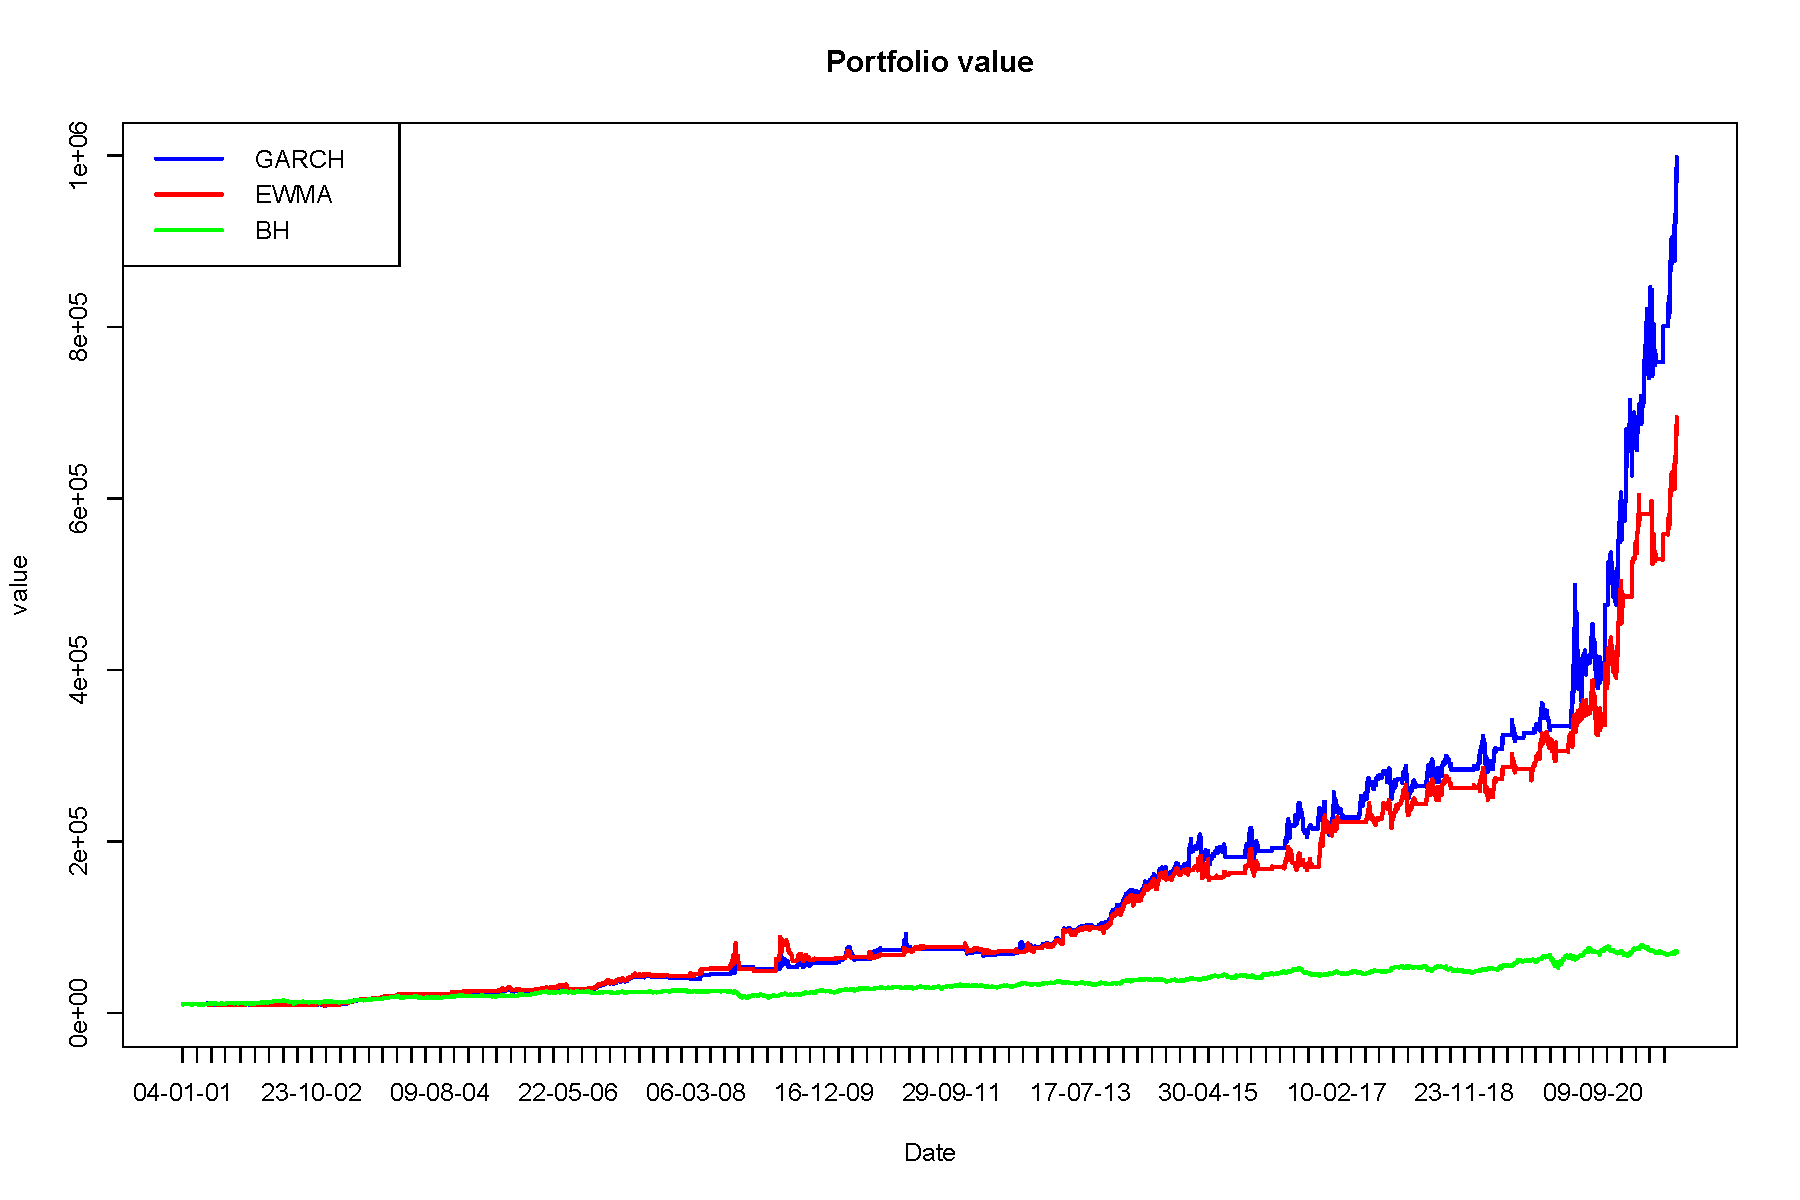
\includegraphics[width=.9\linewidth]{./1.pdf}
\caption[Fig.1]{Portfolio value using different approach}
\end{figure}

\noindent Portfolio value at last trading date: \\
GARCH(1,1):    1486956 USD\\
EWMA:690605 USD\\
Buy and Hold :70415 USD\\
Figure 1 demonstrates the  portfolio value after implementing our investment strategy and buy-and-hold our historical PCA selection in 2000. Blue line indicates our strategy using GARCH(1,1) as the volatility estimate, which outperforms the red lines using EWMA model and green lines(Buy-and Hold). Our strategy using GARCH(1,1) model has result in an around 150 times return from the principal 10000USD. While the EWMA model results in around 70 times of the principal. However Buy and Hold strategy just got 7 times of the principal.
\begin{figure}[H]
\centering
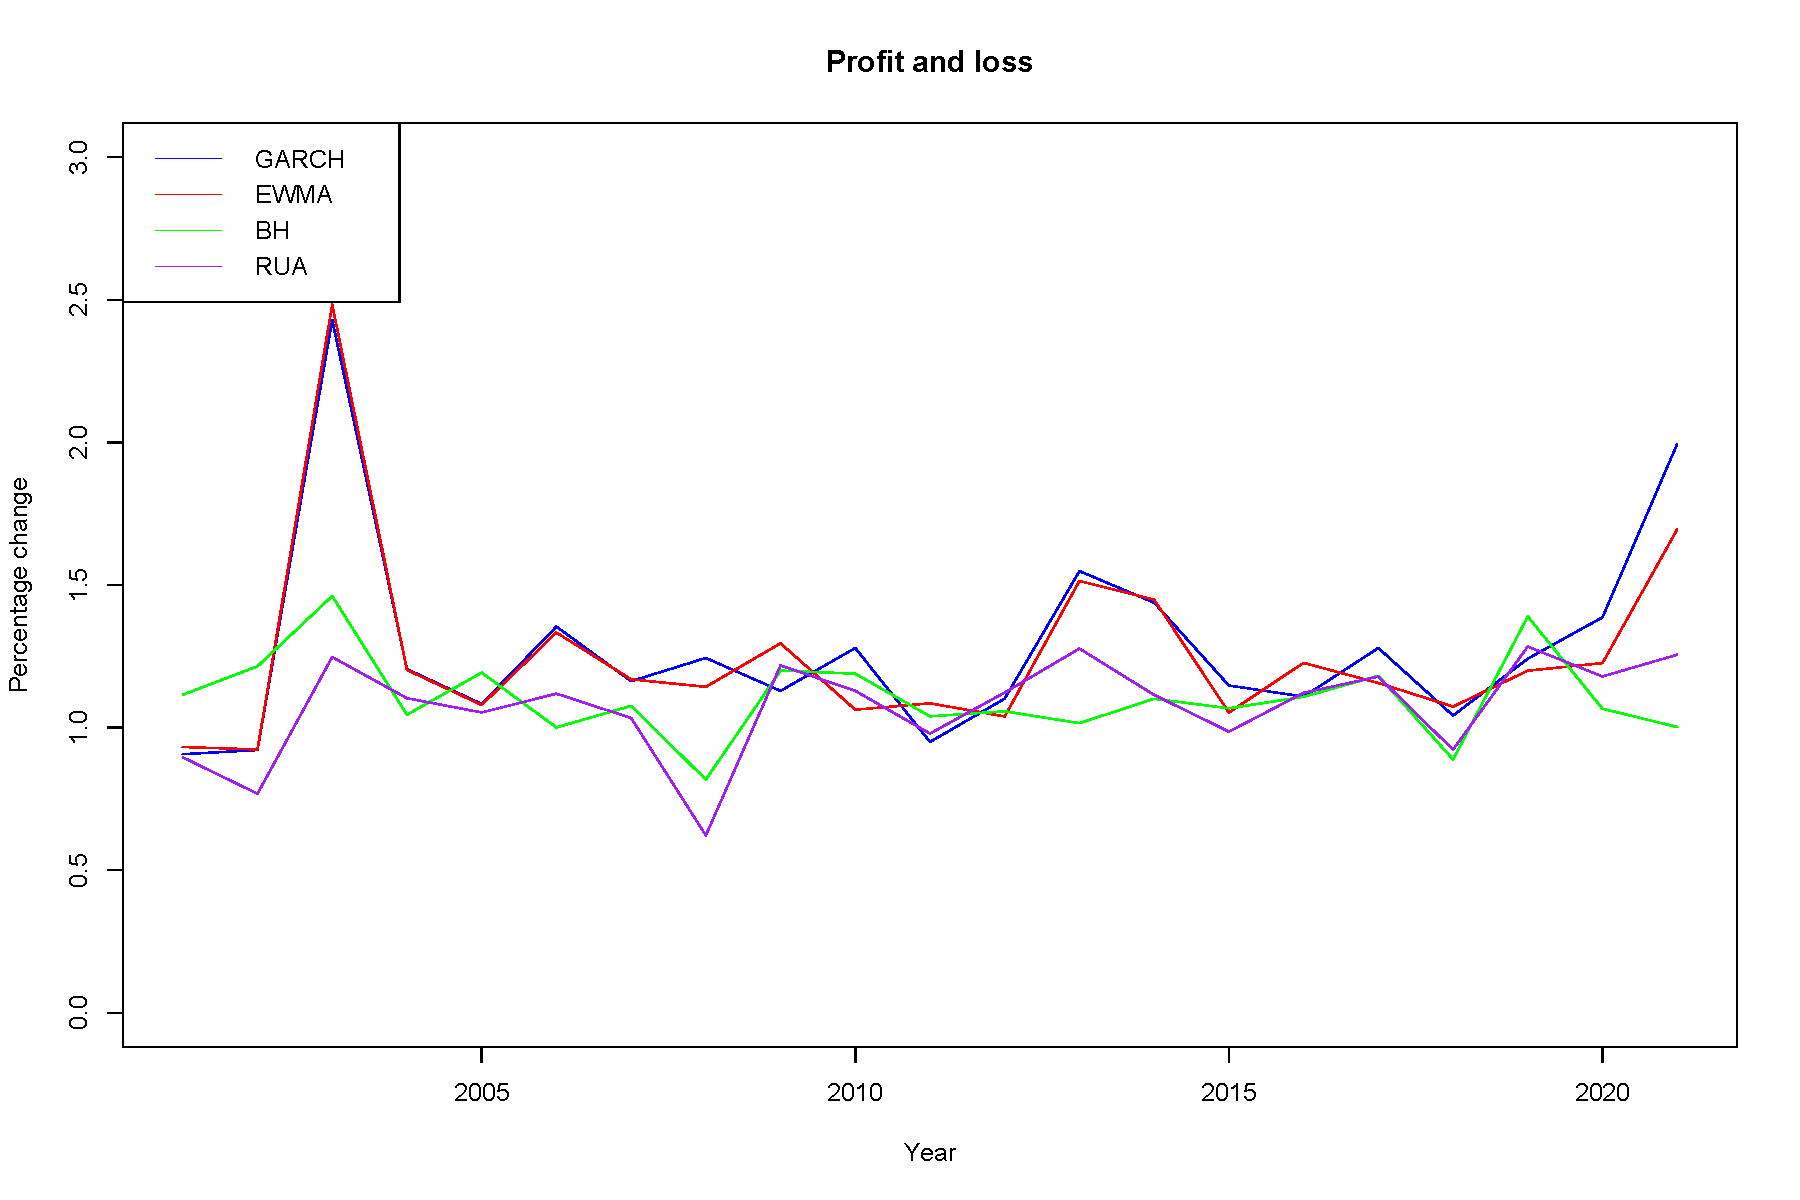
\includegraphics[width=.9\linewidth]{./2.pdf}
\caption[Fig.2]{Year ended profit and loss using different approach}
\end{figure}
\begin{table}[H]
\centering
\begin{tabular}{lllll}
\hline
                          & Garch (\%) & EWMA (\%) & BH (\%) & RUA (\%) \\ \hline
\multicolumn{1}{l|}{2001} & 90.67      & 93.19    & 111.52 & 89.58   \\
\multicolumn{1}{l|}{2002} & 92.13      & 92.33    & 121.49 & 76.81   \\
\multicolumn{1}{l|}{2003} & 242.91     & 248.33   & 146.12 & 124.73  \\
\multicolumn{1}{l|}{2004} & 120.51     & 120.22   & 104.5  & 110.3   \\
\multicolumn{1}{l|}{2005} & 108.27     & 107.93   & 119.27 & 105.3   \\
\multicolumn{1}{l|}{2006} & 135.41     & 133.33   & 100.06 & 111.9   \\
\multicolumn{1}{l|}{2007} & 116.26     & 116.93   & 107.62 & 103.36  \\
\multicolumn{1}{l|}{2008} & 124.41     & 114.28   & 81.76  & 62.19   \\
\multicolumn{1}{l|}{2009} & 112.88     & 129.55   & 119.99 & 121.79  \\
\multicolumn{1}{l|}{2010} & 127.9      & 106.28   & 118.9  & 112.86  \\
\multicolumn{1}{l|}{2011} & 94.97      & 108.51   & 103.95 & 97.91   \\
\multicolumn{1}{l|}{2012} & 110.15     & 103.9    & 105.71 & 112.29  \\
\multicolumn{1}{l|}{2013} & 154.87     & 151.42   & 101.55 & 127.69  \\
\multicolumn{1}{l|}{2014} & 143.8      & 144.86   & 110.1  & 111.46  \\
\multicolumn{1}{l|}{2015} & 114.76     & 105.3    & 106.76 & 98.59   \\
\multicolumn{1}{l|}{2016} & 110.84     & 122.69   & 110.8  & 112.18  \\
\multicolumn{1}{l|}{2017} & 127.91     & 115.64   & 118.16 & 117.88  \\
\multicolumn{1}{l|}{2018} & 104.21     & 107.35   & 88.83  & 92.25   \\
\multicolumn{1}{l|}{2019} & 124.17     & 119.95   & 138.97 & 128.4   \\
\multicolumn{1}{l|}{2020} & 138.67     & 122.62   & 106.61 & 117.94  \\
\multicolumn{1}{l|}{2021} & 199.48     & 169.52   & 100.2  & 125.55  \\ \hline
\end{tabular}
\caption{Year ended percentage of each trading strategy}
\label{tab:2}
\end{table}
Figure 2 and Table 1 show the year ended percentage change for each approach. We can see that most of the year our proposed trading strategies are making profit. For GARCH(1,1), 18 out of 21 years are making profit. The losses have occurred in only 3 out of 21 years. The largest profit was +142.91\% in 2003, and the largest loss was  - 9.33\% in 2001. For EWMA, 19 out of 21 years are making profit. The losses have occurred in only 2 out of 21 years. The largest profit was +148.33\% in 2003, and the largest loss was -7.67\% in 2002. From Figure 2, we can see that most of the years the performance of our proposed trading strategies are better than buy and hold strategy and Russell3000 index. Also, they can prevent losses from the global financial crisis in 2008. The Russell3000 index loss with -37.81\% in 2008, buy and hold strategy loss with -12.24\% in 2008. However, our proposed trading strategies were making profit in 2008.

\begin{table}[H]
\centering
\begin{tabular}{lll}
\hline
\multicolumn{3}{l}{GARCH(1,1)}                         \\
Stocks & Trading frequency & Sector                    \\ \hline
ATI    & 38                & Basic Materials/Resources \\
CENX   & 36                & Basic Materials/Resources \\
CPE    & 32                & Energy Service            \\
CLF    & 30                & Basic Materials/Resources \\
EMKR   & 28                & Technology                \\
MTW    & 28                & Industrial Goods          \\
WRLD   & 28                & Financial Services        \\
YELL   & 28                & Logistics                 \\
MTG    & 26                & Financial Services        \\
GERN   & 24                & Health care               \\ \hline
\end{tabular}
\caption{Most frequently traded stocks using GARCH}
\label{tab:2}
\end{table}

\begin{table}[H]
\centering
\begin{tabular}{lll}
\hline
\multicolumn{3}{l}{EWMA}                               \\
Stocks & Trading frequency & Sector                    \\ \hline
CENX   & 52                & Basic Materials/Resources \\
MTG    & 52                & Financial Services        \\
CLF    & 40                & Basic Materials/Resources \\
SRPT   & 40                & Health care               \\
ATI    & 36                & Basic Materials/Resources \\
MTW    & 36                & Industrial Goods          \\
SNBR   & 36                & Consumer Goods            \\
CPE    & 32                & Energy Service            \\
EMKR   & 32                & Technology                \\
YELL   & 32                & Logistics                 \\ \hline
\end{tabular}
\caption{Most frequently traded stocks using EWMA
}
\label{tab:3}
\end{table}

\begin{table}[H]
\centering
\begin{tabular}{l|ll}
\hline
           & Buy triggered & Sell triggered \\ \hline
GARCH(1,1) & 109           & 108            \\
EWMA       & 131           & 130            \\ \hline
\end{tabular}
\caption{Trading frequency}
\label{tab:4}
\end{table}

\subsection{Interpretation}
\label{sec:orgc722d51}
\subsubsection{Trading frequency}
\label{sec:orgbf3db92}
Table 4 indicates that the number of trades in EWMA model is higher than GARCH(1,1) for about 30 trades, we can interpret that the goodness of using EWMA is easier to be triggered compared to GARCH(1,1). However when we are comparing the most frequent trade in Table 1 and 2 , EWMA trades about two times more than GARCH(1,1) in their most traded stocks.

\subsubsection{Diversification}
\label{sec:org0ef4c10}
Table 2 and 3 highlighted the sectors of the stocks in the correspondent portfolio, the sectors of these most frequently traded stocks are diversified over the portfolio in both GARCH(1,1) and EWMA model, with various types of sectors such as Basic Materials, Technology, Energy service, Financial service, etc. The PCA method extracts the independent components from the index. The good performing stocks and the uncorrelated variables are selected by PCA. The resulting portfolio can perform as principal components of the Russell3000 index, which can be used to represent the financial market and reduce the noise and underperforming stocks.
\subsubsection{Major Market Events}
\label{sec:orgd816dff}

There were two major financial crises included in our project, i.e. during 2008 - 2009 and during 2020. They were worth mentioning as we expected our strategy to outperform even during an economic downturn.

The 2008 to 2009 financial crisis was mainly due to the bursting of the housing bubble in U.S.. At that time, the default rate was high due to the drop in housing prices. Therefore, we assumed that the real estate market and bank stocks would perform worse and we believed that they would be automatically excluded by our trading strategy.

During that period, the return of our trading strategy was 24.41\% and 14.28\% respectively of GARCH and EWMA model. At that time, our strategy had traded 8 times with PCA selected portfolio. They were mainly health care, logistics stocks  These types of stocks could perform well during the financial crisis because they are not correlated to the real estate market.


Simultaneously, the return of Russell3000 falls over 37\%  , much lower than our trading strategy.


On the other hand, the 2020 financial crisis was due to COVID-19. Because of the fear of pandemic, people were pessimistic about the economy and even some risk-free assets faced drop in prices. Therefore, we assumed that some stocks such as luxury goods, aviation, and tourism would perform worse and we believed that they would be automatically excluded by our trading strategy.

During 2020, the return of our trading strategy was 38\% and 22.6\% respectively. The virus affected the stock market mostly during late February to Early April, by our investment strategy, we sold all of our portfolio on 2020-02-04 and 2020-03-05 in GARCH and EWMA model while start buying on 2020-05-18 and 2020-05-04. Our strategy had dodged away the tremendous fall in the crisis and still had a positive return in the whole year.


Simultaneously, the return of buy-and-hold Russell3000 was only 18\%, much lower than our trading strategy.


In short, the simulation proved that our trading strategy, which is a combination of PCA, portfolio optimization, and Kelly's Formula, performs better than the market, no matter whether the economy is in upturn or in downturn.
\section{Conclusion}
\label{sec:orgeda675c}
In this project, we introduce a stock selection method with PCA, a portfolio weighting method with Mean-Variance optimization method, and a trading strategy with Kelly's formula using GARCH model and EWMA method for forecasting. These three techniques combined together to form an optimal trading strategy to compare with buy and hold strategy and Russell3000 index. The testing period is between 2001-01-04 and 2021-11-12. The trading strategy we proposed can outperform the Russell3000 index and buy and hold strategy in the testing period.
\subsection{Limitations}
\label{sec:org408610d}
\begin{enumerate}
\item We proposed that we triggered the buy/sell signal by the threshold that is determined by the overall portfolio return and volatility, if one of the stocks in the portfolio performs badly, we might not able to notice that and change our portfolio

\item Due to the large data size, the total running time of the simulation was long. Meanwhile, since we run through all the trading days with GARCH(1,1) and EWMA,  the for-loops in the program have further lengthened the running time.

\item In our project, we downloaded all required data first then did the simulation. However, in practice, data may need to be updated daily. It is daily additional work and time is needed to download all the components’ price in Russell300 to start the analysis every day.

\item Liquidity,  the simulation assumed that stock could be bought or sold immediately. But in the real world, there may be a time lag for the trading to be done, especially if the trading volume for that stock is not high. This may result in a reduction of return as price may have changed during the time lag. On the contrary, the buy-and-hold strategy would not have this problem because it only buys or sells once in the trading period.
\end{enumerate}

\subsection{Imporvements}
\label{sec:orgd8b4ebf}
\begin{enumerate}
\item To shorten the running time in practice, we could choose only one among the GARCH(1,1) and EWMA volatility estimation methods. From the simulation, we could see that the portfolio return calculated by GARCH(1,1) and EWMA had very similar results from the start of the simulation period to the end of it.

\item The number of stocks in the pool could be smaller. In our simulation, we picked all components of Russell3000 into the pool for PCA. In practice, however, we may choose fewer stocks to put into the pool. This could shorten the time for data collection and extraction. It is suggested that the market value of stocks to be not too small, for example at least greater than 1 billion, and that the pool should contain various types of stocks so that the strategy would be able to cater different economic situations. It is important to note that since the pool is smaller, maybe we need to update the stocks in the pool regularly for more accurate results. There are trade-offs between accuracy and data set size.

\item To lower the chance that the stock is too hard to be traded due to a small trading volume in the market, we may avoid choosing less popular stocks.

\item Short Selling can be considered to be added to the strategy by selecting the least loadings in the PCA computed, also as our buy/sell strategy is based on volatility, short selling can also be possible in our strategy.
\end{enumerate}
\section*{References}
\label{sec:org5b75a77}
\noindent J.P. Morgan. (1996). Risk Metrics: technical document. New York, N.Y.

\noindent Rea, William \& Rea, Alethea \& Yang, Libin. (2015). Stock Selection with Principal Component Analysis. 10.13140/2.1.2220.8805.
\end{document}
